\documentclass{beamer}
\setbeamertemplate{navigation symbols}{} % eliminate navigation bar
\usetheme{CambridgeUS}

\usefonttheme{structurebold}
% Arch Linux Color Theme
\definecolor{arch}{RGB}{23,147,209}
\usecolortheme[named=arch]{structure}
\usecolortheme{whale}
\setbeamercolor{frametitle}{bg=arch!80!black}
\setbeamercolor{title}{bg=arch!90!black}

%% SET BEAMER TEMPLATE
%\setbeamertemplate{headline}

\usepackage{lmodern}
\usepackage{ngerman}
\usepackage[latin1]{inputenc}
\usepackage[naustrian,ngerman]{babel}

\usepackage{listings}
\lstset{basicstyle=\tiny\ttfamily,
  frame=single}
\usepackage[squaren,thinqspace,thinspace]{SIunits}

\beamersetuncovermixins{\opaqueness<1>{25}}{\opaqueness<2->{15}}


%% META INFORMATION ABOUT DOCUMENT
% \title[short]{long}
% short argument is used in places where there is little space
% long is used on the title slide

\title[Impedanzspektrometer]{mini Impedanzspektrometer mit dem AD5933}
\subtitle{Bachelorarbeit SS2014}
\institute[]{Institut f�r Mikroelektronik und Mikrosensorik \\ Johannes-Kepler-Universit�t Linz}

\subject{AD5933 Impedanzspektrometer}

% ENTER YOUR NAME, SHORT VERSION FOR FOOTER
\author[Feichtinger]{Peter Feichtinger\texorpdfstring{\\}{, } Betreuer: DI Stefan Clara} % Variante: \and

\date{16. Dezember 2014}


\begin{document}

%% TITLE PAGE
\begin{frame}
  \titlepage
\end{frame}

% for longer presentations table of contents is useful
% \begin{frame}
%    \frametitle{Outline} 
%    \tableofcontents          % optional: [pausesections]
% \end{frame}


\section{Entwicklung}  % always defined outside a frame, optional short argument
\begin{frame}[t]
  \frametitle{Einleitung}

  \begin{columns}
    \begin{column}{0.6\textwidth}
      \begin{itemize}
        \item Kompakte und preiswerte M�glichkeit zur Messung von Impedanzspektren
        \item Basierend auf dem STM32F4 Discovery Board und Analog Devices AD5933 \emph{Impedance Converter} IC
        \item Bedienung �ber MATLAB und virtuelle serielle Schnittstelle
      \end{itemize}
      \vspace{2cm}
    \end{column}
    
    \begin{column}{0.35\textwidth}
      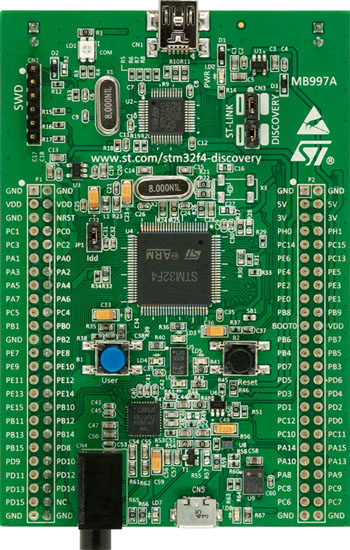
\includegraphics[height=15em]{bilder/stm32.jpg} \\
      \footnotesize{STM32F4 Discovery Board}
    \end{column}
  \end{columns}
\end{frame}

\begin{frame}[t]
  \frametitle{Hardware}
  
  \begin{itemize}
    \item Externes Analog-Frontend zum AD5933 mit 4-Leiter Messung
    \item Analog-Multiplexer f�r mehrere Ausg�nge
    \item Austauschbare Kalibrierwiderst�nde
  \end{itemize}
  
  \vspace{1em}
  \centering
  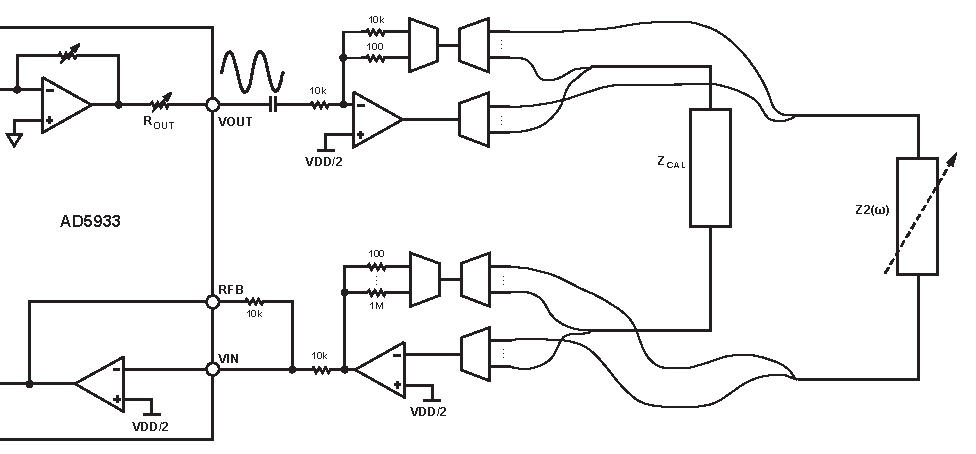
\includegraphics[height=11.5em]{bilder/schem_afe.pdf} \\
    \footnotesize{Schaltung des Analog-Frontend}
\end{frame}

\begin{frame}[t]
  \frametitle{Hardware}
  
  \begin{itemize}
    \item Gr��e von $ 10 \times 14 $\,cm
    \item Stromversorgung �ber USB oder DC-Stecker
    \item EEPROM zum Speichern von Einstellungen
  \end{itemize}
  
  \vspace{1em}
  \centering
  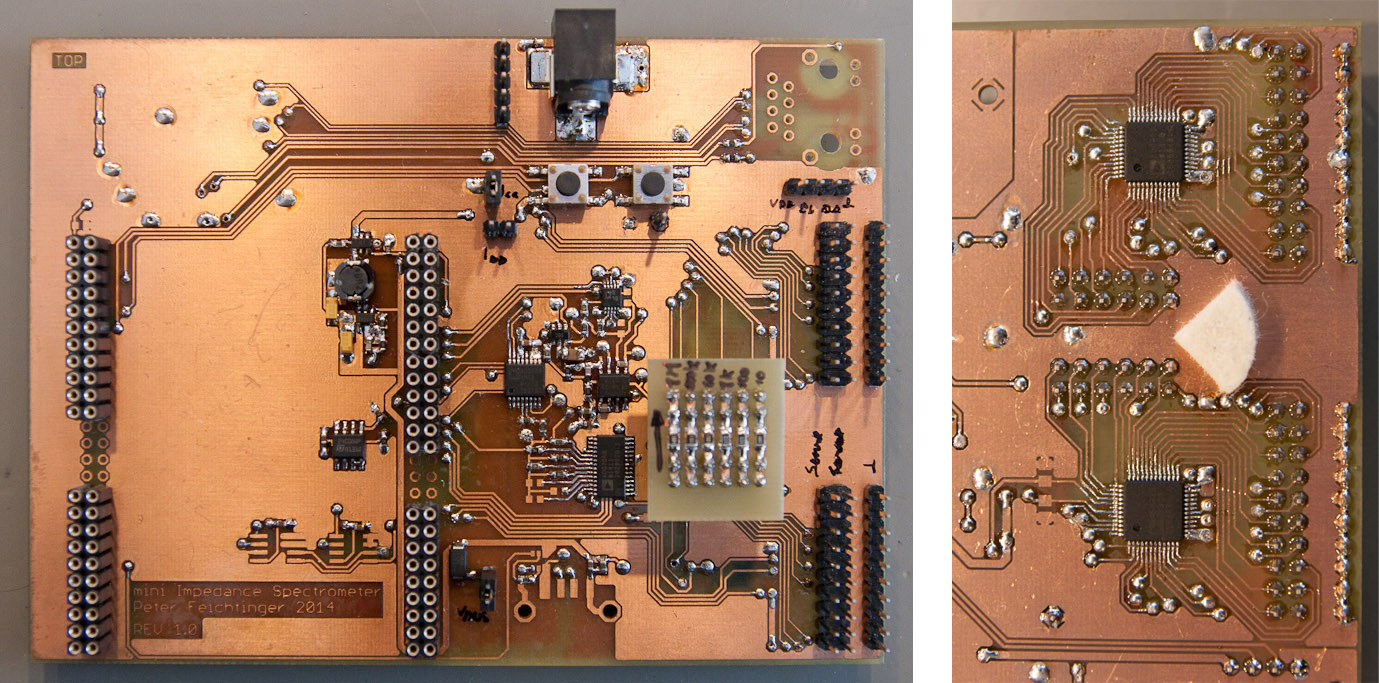
\includegraphics[height=11.5em]{bilder/pcb_rev1.jpg} \\
    \footnotesize{Erste Version der Platine}
\end{frame}

\begin{frame}[t]
	\frametitle{Firmware}
  
  \begin{itemize}
    \item Programmiert in C
    \item ST HAL Bibliothek f�r leichte Portierbarkeit
    \item Modularer Aufbau f�r gute Erweiterbarkeit
    \item Konfiguration in EEPROM gespeichert
    \begin{itemize}
      \item Aktuelle Einstellungen
      \item Best�ckung von Widerst�nden
      \item Ethernet MAC-Adresse
    \end{itemize}
  \end{itemize}
\end{frame}


\section{Verwendung}
\begin{frame}[c,fragile=singleslide]
  \frametitle{Bedienung}
  
  \begin{columns}
    \begin{column}{0.5\textwidth}
      \begin{itemize}
        \item Konfiguration �ber Konsoleninterface
        \item Auslesen der Werte in verschiedenen Formaten
        \item MATLAB Funktionen zur automatisierten Steuerung
      \end{itemize}
      \vspace{2cm}
    \end{column}
    
    \begin{column}{0.45\textwidth}
      \begin{lstlisting}
board set --start=10k --stop=20k
board set --steps=10 --voltage=400
board calibrate 100
OK
board start 0
OK
board read
Frequency Magnitude Angle
10000 11.5255 1.10659
11000 14.0605 1.17955
12000 18.1948 1.13351
13000 24.6496 1.04903
14000 35.7221 0.883436
15000 54.9023 0.512685
16000 68.6387 -0.185134
17000 52.3116 -0.825151
18000 36.2655 -1.12627
19000 27.0367 -1.27099
20000 21.4698 -1.35018
      \end{lstlisting}
    \end{column}
  \end{columns}
\end{frame}

\begin{frame}[c]
  \frametitle{Ergebnisse}
  
  \begin{itemize}
    \item Gute Ergebnisse mit niedrigen ohmschen Widerst�nden
  \end{itemize}
  
  \centering
  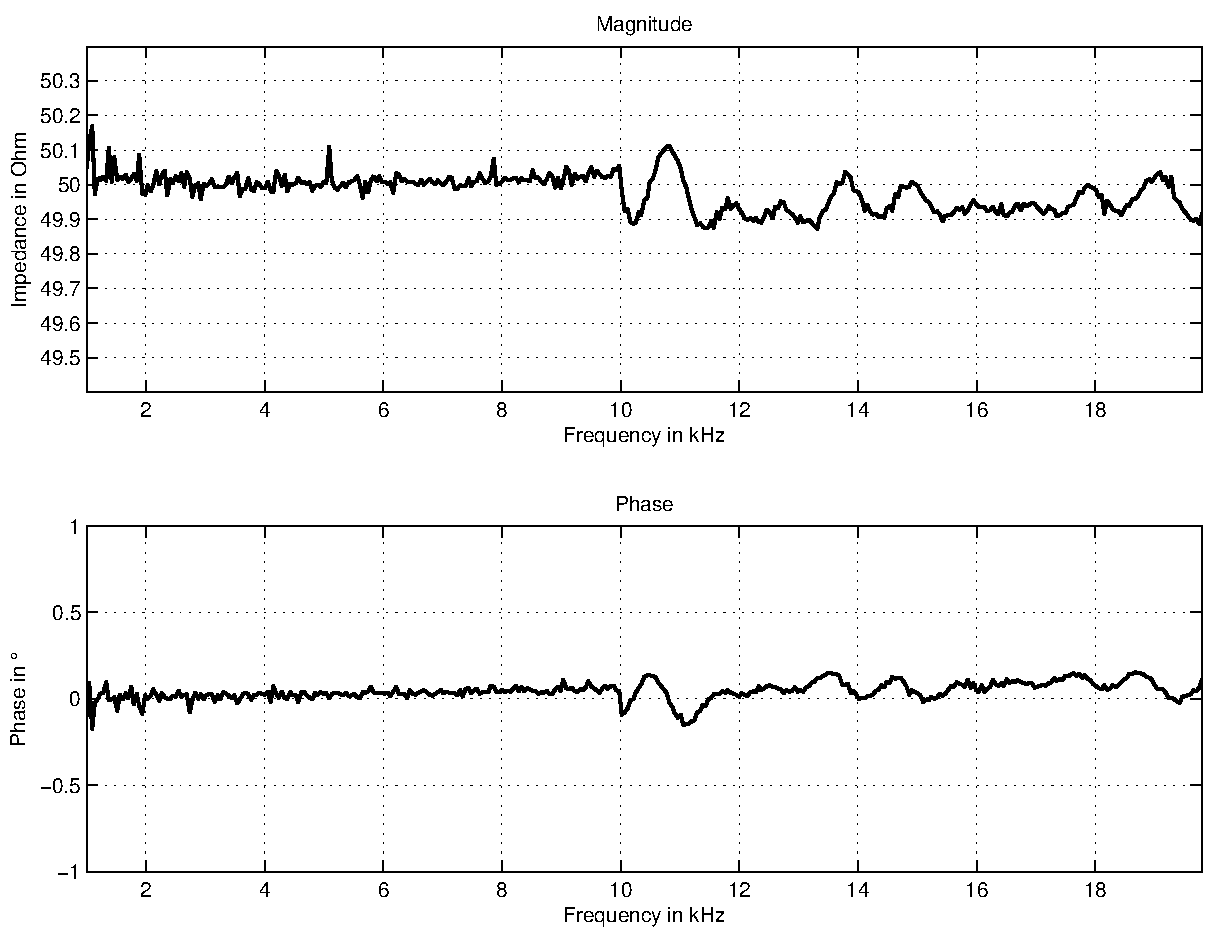
\includegraphics[height=16em]{bilder/49r9.pdf} \\
    \footnotesize{\unit{49.9}{\ohm} Widerstand: \unit{\pm 1}{\%} und \unit{\pm 1}{\degree}}
\end{frame}

\begin{frame}[c]
  \frametitle{Ergebnisse}
  
  \begin{itemize}
    \item Brauchbare Ergebnisse mit hohen ohmschen Widerst�nden
  \end{itemize}
  
  \centering
  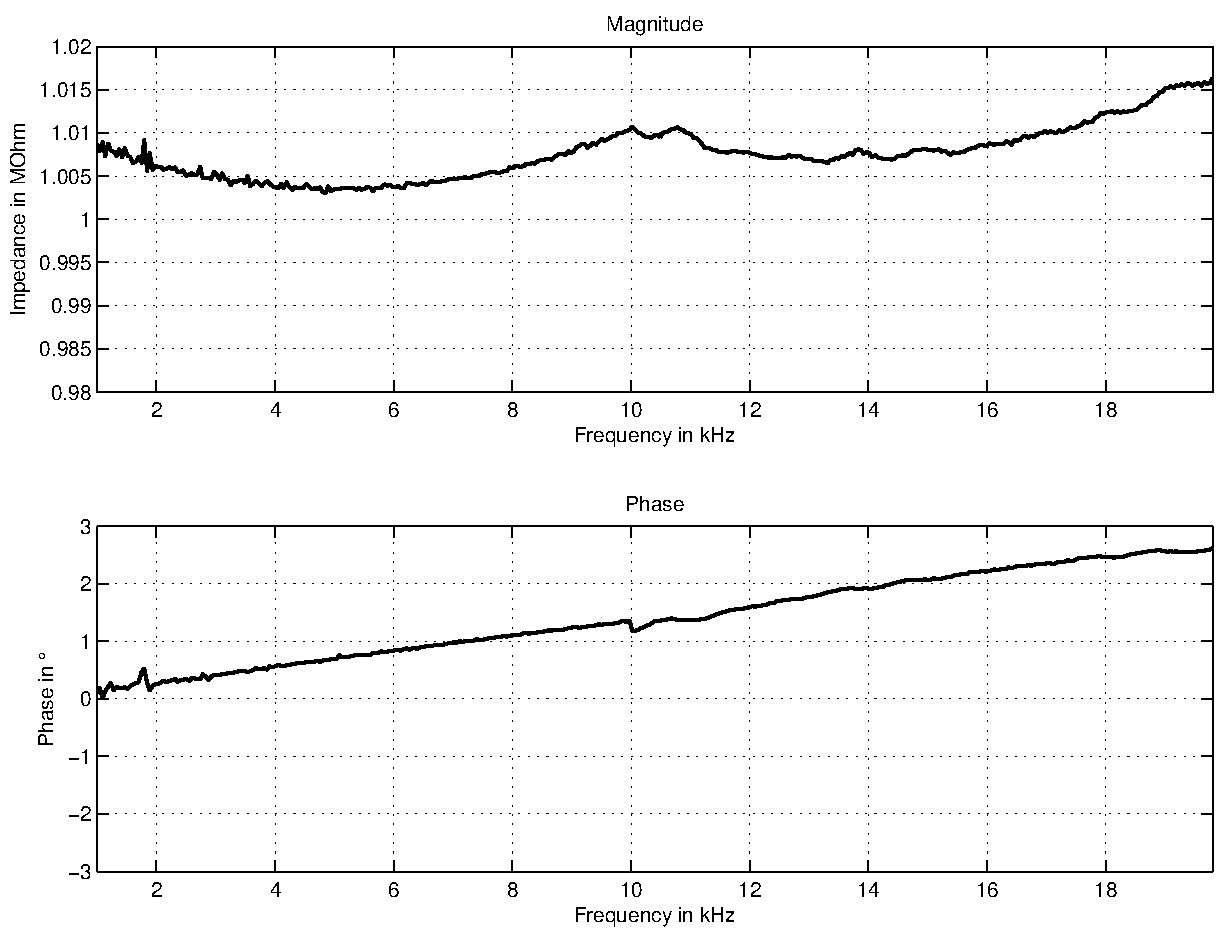
\includegraphics[height=16em]{bilder/1M.pdf} \\
    \footnotesize{\unit{1}{\mega\ohm} Widerstand: \unit{\pm 2}{\%} und \unit{\pm 3}{\degree}}
\end{frame}

\begin{frame}[c]
  \frametitle{Ergebnisse}
  
  \begin{itemize}
    \item Unbrauchbar bei kleinen gemischten Impedanzen
  \end{itemize}
  
  \centering
  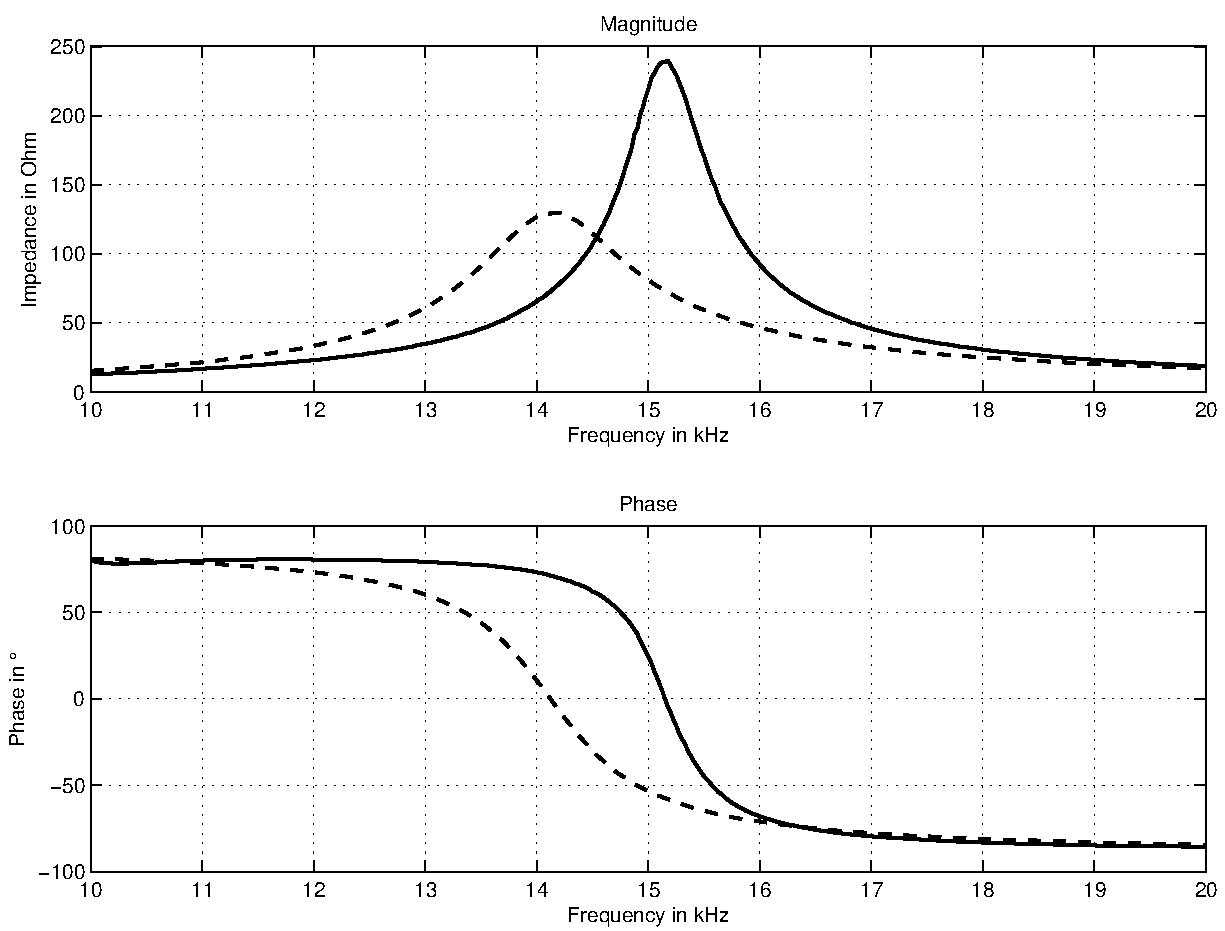
\includegraphics[height=16em]{bilder/S22.pdf} \\
    \footnotesize{Parallelschwingkreis: $ \unit{100}{\micro\henry} \,\|\, \unit{1}{\micro\farad} $}
\end{frame}

\begin{frame}[c]
  \frametitle{Verbesserungen}
  
  \begin{columns}
    \begin{column}{0.5\textwidth}
      \begin{itemize}
        \item Robusteres Analog-Frontend
        \item Autoranging implementieren
        \item Ethernet und USB Schnittstellen implementieren
        \item Genauigkeit verbessern
      \end{itemize}
      \vspace{2cm}
    \end{column}
    
    \begin{column}{0.45\textwidth}
      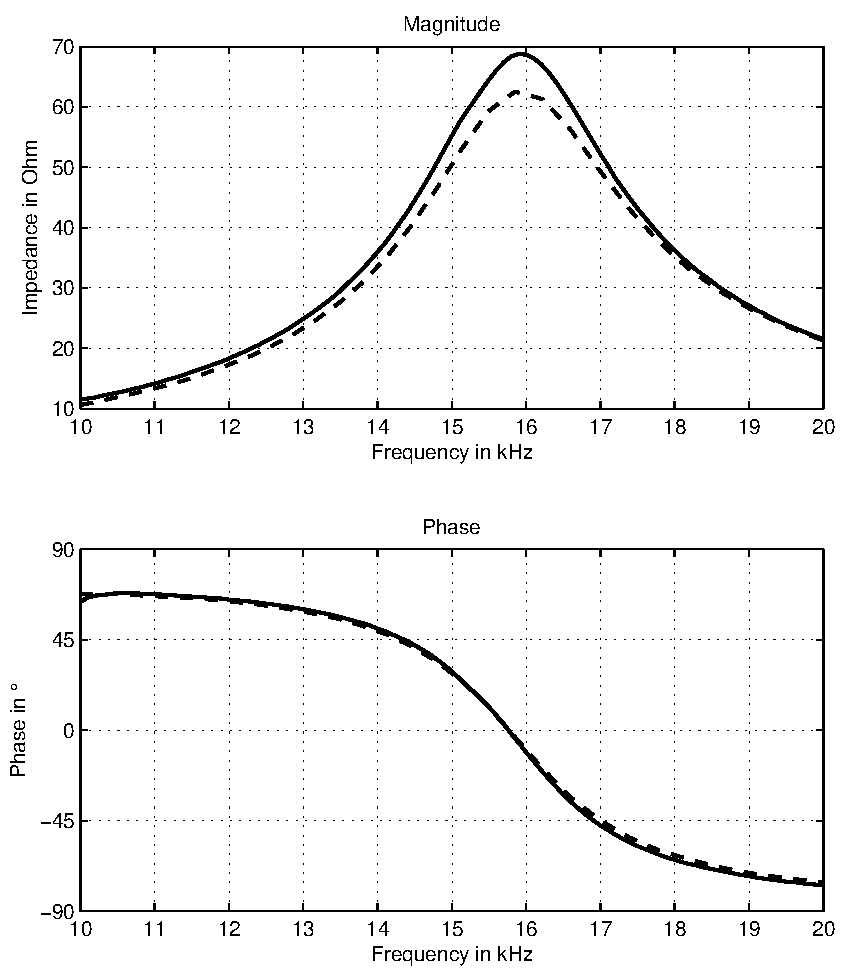
\includegraphics[height=16em]{bilder/lcp_fail.pdf}
    \end{column}
  \end{columns}
\end{frame}

\begin{frame}
  \centering
  Noch Fragen?
\end{frame}


\end{document}